\chapter{Logistic regression}
\label{chap-logistic}


%%%%%%%%%%%%%%%%%%%%%%%%%%%%%%%%%%%%%%%%%%%%%%%%%%%%%%%%%%%%%%%%%%%%%%%%%%%%%
\section{A new hypothesis class: linear logistic classifiers}

For classification, it is natural to make predictions in $\{+1, -1\}$
and use the $0-1$ loss function.   However, even for simple linear
classifiers, it is very difficult to
find values for $\theta, \theta_0$ that minimize simple training error
\[J(\theta, \theta_0) = \frac{1}{n} \sum_{i=1}^n \mathcal{L}(\text{sign}(\theta^T\ex{x}{i} + \theta_0),
  \ex{y}{i})\;\;.\] This problem is NP-hard, which probably
\note{The ``probably'' here is not because we're too lazy to look it
  up, but actually because of a fundamental unsolved problem in
  computer-science theory, known as ``P vs. NP.''}
implies
that solving the most difficult instances of this problem would
require computation time {\em exponential} in the number of training
examples, $n$.

What makes this a difficult optimization problem is its lack of
``smoothness'':
\begin{itemize}
\item There can be two hypotheses, $(\theta, \theta_0)$  and
  $(\theta', \theta_0')$, where
  one is closer in parameter space to the optimal parameter values
  $(\theta^*, \theta_0^*)$, but they make the same number of
  misclassifications so they have the same $J$ value.
\item All predictions are categorical:  the classifier can't express a
  degree of certainty about whether a particular input $x$ should have
  an associated value $y$.
\end{itemize}
For these reasons, if we are considering a hypothesis $\theta,\theta_0$
that makes five incorrect predictions, it is difficult to see how we
might change $\theta,\theta_0$ so that it will perform better, which
makes it difficult to design an algorithm that searches through the
space of hypotheses for a good one.

For these reasons, we are going to investigate a new hypothesis class:
{\em linear logistic classifiers}.   These hypotheses are still
parameterized by a $d$-dimensional vector $\theta$ and a scalar
$\theta_0$, but instead of making predictions in $\{+1, -1\}$, they
generate real-valued outputs in the interval $(0, 1)$. A linear
logistic classifier has the form 
\[h(x; \theta, \theta_0) = \sigma(\theta^T x + \theta_0)\;\;.\]
This looks familiar!  What's new?

The {\em logistic} function, also known as the {\em sigmoid} function, 
is defined as
\[\sigma(z) = \frac{1}{1+e^{-z}}\;\;,\] and plotted below, as a
function of its input $z$.
Its output can be interpreted as a probability, because for any value of
$z$ the output is in $(0, 1)$.

\begin{center}
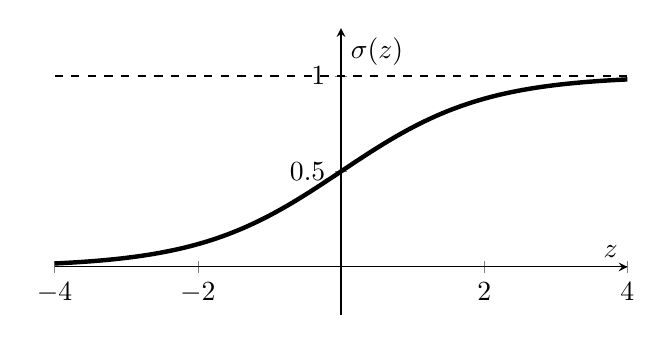
\begin{tikzpicture}
\begin{axis}[
  axis lines=middle,
  % axis equal image,
  scale only axis,
  width=0.6\textwidth,
  height=0.3\textwidth,
    xmin=-4, xmax=4,
    ymin=-0.25, ymax=1.25,
    xlabel={$z$}, ylabel={$\sigma(z)$},
]
\addplot [domain=-4:4, samples=100, ultra thick] {1/(1+exp(-x))};
\addplot [domain=-4:4, samples=2, dashed] {1};
\addplot [domain=-4:4, samples=2, dashed] {0};
\end{axis}
\end{tikzpicture}
\end{center}

\question{Convince yourself the output of $\sigma$ is always in the
  interval $(0, 1)$.  Why can't it equal 0 or equal 1?  For what value
of $z$ does $\sigma(z) = 0.5$?}

What does a linear logistic classifier (LLC) look like?   Let's consider the
simple case where $d = 1$, so our input points simply lie along the
$x$ axis.  The plot below shows LLCs for three different parameter
settings: $\sigma(10x + 1)$, $\sigma(-2x + 1)$, and $\sigma(2x - 3).$
\begin{center}
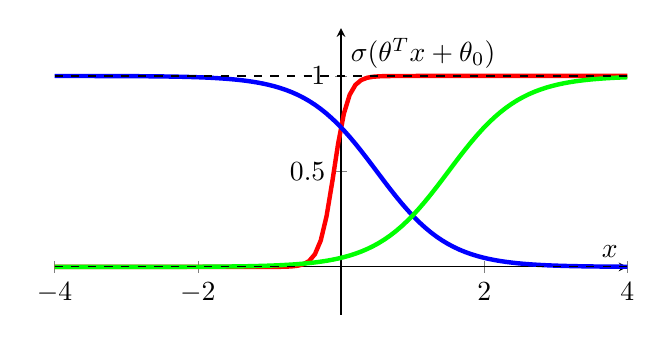
\begin{tikzpicture}
\begin{axis}[
  axis lines=middle,
  % axis equal image,
  scale only axis,
  width=0.6\textwidth,
  height=0.3\textwidth,
    xmin=-4, xmax=4,
    ymin=-0.25, ymax=1.25,
    xlabel={$x$}, ylabel={$\sigma(\theta^T x + \theta_0)$},
]
\addplot [domain=-4:4, samples=100, ultra thick, red] {1/(1+exp(-(10*x + 1)))};
\addplot [domain=-4:4, samples=100, ultra thick, blue] {1/(1+exp(-(-2*x
  + 1)))};
\addplot [domain=-4:4, samples=100, ultra thick, green] {1/(1+exp(-(2*x
  - 3)))};
\addplot [domain=-4:4, samples=2, dashed] {1};
\addplot [domain=-4:4, samples=2, dashed] {0};
\end{axis}
\end{tikzpicture}
\end{center}
\question{Which plot is which?  What governs the steepness of the
  curve?  What governs the $x$ value where the output is equal to
  0.5?}

But wait!  Remember that the definition of a classifier from
chapter~\ref{chap-classification} is that it's a mapping from $\R^d
\rightarrow \{-1, +1\}$ or to some other discrete set.  So, then, it
seems like an LLC is actually not a classifier! 

Given an LLC, with an output value in $(0, 1)$, what should we do if
we are forced to make a prediction in $\{+1, -1\}$?  A default answer
is to predict $+1$ if $\sigma(\theta^T x + \theta_0) > 0.5$ and $-1$
otherwise.  The value $0.5$ is sometimes called a {\em prediction
  threshold}.

In fact, for different problem settings, we might prefer to pick a
different prediction threshold.  The field of {\em decision theory}
considers how to make this choice from the perspective of Bayesian
reasoning.  For example, if the consequences of predicting $+1$ when
the answer should be $-1$ are much worse than the consequences of
predicting $-1$ when the answer should be $+1$, then we might set the
prediction threshold to be greater than $0.5$.

\question{Using a prediction threshold of 0.5, for what values of $x$
  do each of the LLCs shown in the figure above predict $+1$?}

When $d = 2$, then our inputs $x$ lie in a two-dimensional space with
axes $x_1$ and $x_2$, and the output of the LLC is a surface, as shown
below, for $\theta = (1, 1), \theta_0 = 2$.

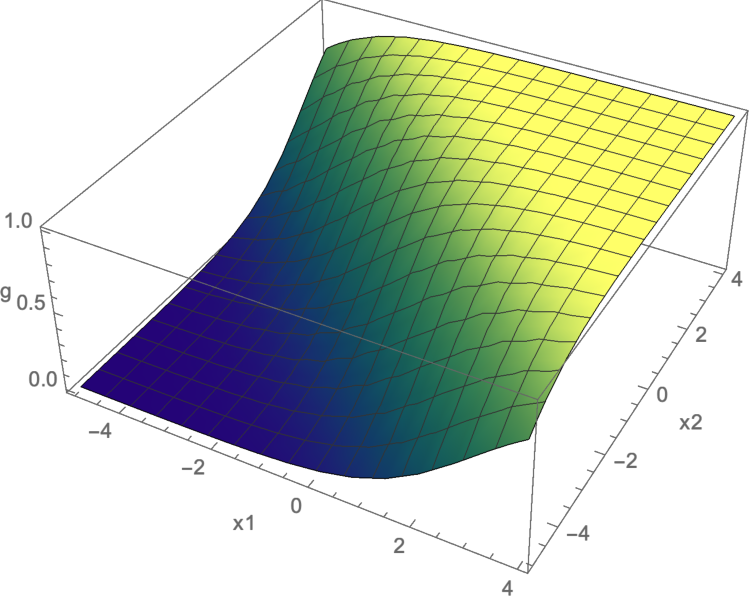
\includegraphics[width=0.7\textwidth]{figures/logreg3d}

\question{Convince yourself that the set of points for which
  $\sigma(\theta^T x + \theta_0) = 0.5$, that is, the separator
  between positive and negative predictions with prediction threshold
  $0.5$ is a line in $(x_1, x_2)$ space. What particular line is it
  for the case in the figure above?
  How would the plot change for $\theta = (1, 1)$, but now
  with $\theta_0 = -2$? For $\theta = (-1, -1), \theta_0 = 2$?}

%%%%%%%%%%%%%%%%%%%%%%%%%%%%%%%%%%%%%%%%%%%%%%%%%%%%%%%%%%%%%%%%%%%%%%%%%%%%%
\section{Loss function for logistic classifiers}

\label{logistic}
Recall that optimization is a key approach to solving machine learning
problems; this also applies to logistic regression, as we can see by
defining a lass function for this problem.  Recall that a common loss function
is the 0-1 loss, introduced in Chapter~\ref{chap-intro}:
\[ L_{01}(h(x; \Theta), y) =
  \begin{cases}
    0 & \text{ if } y = h(x; \Theta)\\
    1 & \text{ otherwise}
  \end{cases}\;\;,
\]
which gives a value of 0 for a correct prediction, and a 1 for an
incorrect prediction.  In the case of linear separators, this becomes:
\[ L_{01}(h(x;\theta, \theta_0), y) =
  \begin{cases}
    0 & \text{ if } y(\theta^Tx + \theta_0) > 0 \\
    1 & \text{ otherwise}
  \end{cases}\;\;.
\]


%
For logistic regression, we have defined a class, LLC, of hypotheses whose outputs are in $(0, 1)$, 
but we have training data with $y$ values  in $\{+1, -1\}$.  How
can we define a loss function?  Intuitively, we would like to have
{\em low loss if we assign a low probability to the incorrect class.}
We'll define a loss function, called {\em negative log-likelihood} (NLL),
that does just this.  In  addition, it has the cool property that it
extends nicely to the case where we would like to classify our inputs
into more than two classes.

In order to simplify the description, we will assume that (or transform so that) the labels
in the training data are $y \in \{0, 1\}$, enabling them to be
interpreted as probabilities of being a member of the class of
interest.  \note{\bf Remember to be sure your $y$
  values have this form if you try to learn an LLC using NLL!|}
We would like to pick the parameters of our classifier to maximize the
probability assigned by the LCC to the correct $y$ values, as
specified in the training set.  Letting guess $\ex{g}{i} =
\sigma(\theta^T\ex{x}{i} + \theta_0)$, 
that probability is
\begin{equation*}
 \prod_{i = 1}^n \begin{cases} \ex{g}{i} & \text{if $\ex{y}{i} =
    1$}  \\ 1 - \ex{g}{i} & \text{otherwise}
\end{cases}\;\;,
\end{equation*}
under the assumption that our predictions are independent.  This can
be cleverly rewritten, when $\ex{y}{i} \in \{0, 1\}$, as
\begin{equation*}
 \prod_{i = 1}^n {\ex{g}{i}}^{\ex{y}{i}}(1 - \ex{g}{i})^{1 - \ex{y}{i}}\;\;.
\end{equation*}
\question{Be sure you can see why these two expressions are  the
  same.}

Now, because products are kind of hard to deal with, and because the
log function is monotonic, the $\theta, \theta_0$ that maximize the
log of this quantity will be the same  as the $\theta, \theta_0$ that
maximize the original, so we can try to maximize
\begin{equation*}
  \sum_{i = 1}^n  \left( {\ex{y}{i}}\log {\ex{g}{i}} +
            (1 - \ex{y}{i})\log(1 - \ex{g}{i})\right)\;\;. 
\end{equation*}
We can turn the maximization problem above into a minimization problem by taking the negative
of the above expression, and write in terms of minimizing a loss
\begin{equation*}
 \sum_{i = 1}^n \mathcal{L}_\text{nll}(\ex{g}{i}, \ex{y}{i})
\end{equation*}
where $\mathcal{L}_\text{nll}$ is the {\em negative log-likelihood}
loss function:
\begin{equation*}
\mathcal{L}_\text{nll}(\text{guess},\text{actual}) = 
-\left(\text{actual}\cdot \log (\text{guess}) + (1 - \text{actual})\cdot\log (1 -
  \text{guess})\right) \;\;.
\end{equation*}
This loss function is also sometimes referred to as the {\em log loss}
or {\em cross entropy}. \note{You can use any base for the logarithm
  and it won't make any real difference.  If we ask you for numbers,
  use log base $e$.}

\section{Logistic classification as optimization}

We can finally put all these pieces together and develop an objective
function for optimizing regularized negative log-likelihood for a
linear logistic classifier. \note{That's a lot of fancy words!}  In
  fact, this process is usually called ``logistic regression,'' so
  we'll call our objective $J_\text{lr}$, and define it as
\[J_\text{lr}(\theta, \theta_0; {\cal D}) =
  \left(\frac{1}{n} \sum_{i=1}^n
    \mathcal{L}_\text{nll}(\sigma(\theta^T \ex{x}{i} + \theta_0), \ex{y}{i})\right) +
     \lambda \norm{\theta}^2\;\;.\]
\question{Consider the case of linearly separable data.   What will
  the $\theta$ values that optimize this objective be like if
  $\lambda = 0$?   What will they be like if $\lambda$ is very big?
  Try to work out an example in one dimension with two data points.}

%%% Local Variables:
%%% mode: latex
%%% TeX-master: "top"
%%% End:
